\documentclass[a4paper,11pt,bigheadings,headsepline,titlepage,liststotoc,idxtotoc,bibtotoc,bibliography=totocnumbered]{scrartcl}
\def\ThesisAuthorGivenName{Per}
\def\ThesisAuthorSurname{Bernhardt}
\def\ThesisAuthor{\ThesisAuthorGivenName\  \ThesisAuthorSurname}
\def\ThesisAuthorAddress{Schumannstr. 115 \\ 53113 Bonn}
\def\ThesisExternalCompany{}
\def\ThesisKeywords{}
\def\ThesisLocation{Sankt Augustin}
\def\ThesisPubDate{\today}
\def\ThesisSubject{}
\def\ThesisStudyCourse{Computer Science}
\def\ThesisStudyCourseGerman{Informatik}
\def\ThesisSubjectType{Exposé}
\def\ThesisSupervisorFirst{Christoph Tornau}
\def\ThesisSupervisorSecond{Prof. Dr. Simone Bürsner}
\def\ThesisSupervisorExternal{}
\def\ThesisTitleFirstLine{Testdatenmanagement}
\def\ThesisTitleSecondLine{für automatische Funktionstests}
\def\ThesisTitleThirdLine{bei Chefkoch.de}
\def\ThesisTitle{\ThesisTitleFirstLine\ \ThesisTitleSecondLine\ \ThesisTitleThirdLine}
\def\ThesisTitleMultiLine{\ThesisTitleFirstLine\linebreak{}\ThesisTitleSecondLine\linebreak{}\ThesisTitleThirdLine}
\def\ThesisType{Bachelor}

\usepackage{aussehen/hbrs-inf}
\usepackage{minted}

\newminted{gherkin}{frame=single,framesep=0.5cm}
\newminted{php}{frame=single,framesep=0.5cm}
\newminted{docker}{frame=single,framesep=0.5cm}
\newminted{json}{frame=single,framesep=0.5cm}
\newminted{ruby}{frame=single,framesep=0.5cm}
\newminted{yaml}{frame=single,framesep=0.5cm}

\newcommand{\externalcode}[2]{\inputminted[frame=single,framesep=0.5cm]{#1}{#2}}

\newcommand{\secDir}{abschnitte}
\begin{document}
\begin{spacing}{1}
  \pagenumbering{roman}

\pagestyle{empty}
\begin{titlepage}
\begin{Large}
\begin{flushleft}
\makebox[11cm][c]{
\parbox[c]{2.5cm}{\includegraphics[height=4ex]{bilder/fhlogo.pdf}\vspace{1.40cm}}
\parbox[c]{12.0cm}{\begin{flushleft}
\small{\textbf{Hochschule\linebreak{}Bonn-Rhein-Sieg}\linebreak{}\textit{University of Applied Sciences}\linebreak{}\linebreak{}\textbf{Fachbereich \ThesisStudyCourseGerman}\linebreak{}\textit{Department of \ThesisStudyCourse}}
\end{flushleft}}}
\end{flushleft} 
\end{Large}

\vspace{0.150\textheight}
\begin{center}
 \begin{Huge}\textbf{\ThesisSubjectType}\end{Huge}\\
 \vspace{2em}
 \begin{Large}im \ThesisType-Studiengang \ThesisStudyCourse\end{Large}
 \vspace{0.10\textheight}\\
 \begin{Huge} \textbf{\ThesisTitleMultiLine}
\end{Huge}\\
 \vspace{2em}
 \begin{Large}\textbf{von} \end{Large}\\
 \vspace{1em}
 \begin{Large}\textbf{\ThesisAuthor}\end{Large}\\
\end{center}
\vspace{0.100\textheight}

\begin{Large}
\begin{flushleft}
\begin{tabular}{ll}
Betreuer: & \ThesisSupervisorFirst \\
Zweitbetreuer: & \ThesisSupervisorSecond \\
%Externer Betreuer: & \ThesisSupervisorExternal \\
%~ & \ThesisExternalCompany \\
%~ & \\
Eingereicht am: & \ThesisPubDate
\end{tabular} 
\end{flushleft}
\end{Large}
\end{titlepage}

\end{spacing}

\pagestyle{Hauptteil}

\section*{Erklärung}
\ThesisAuthor \\
\ThesisAuthorAddress \\
\newline
Hiermit erkläre ich, dass ich die vorliegende Arbeit selbst angefertigt habe; die aus fremden Quellen direkt oder indirekt übernommenen Gedanken sind als solche kenntlich gemacht.
\newline
Die Arbeit wurde bisher keiner Prüfungsbehörde vorgelegt und auch noch nicht veröffentlicht.
\newline


\begin{tabular}{ll}
................................ & ................................ \\ 
Ort, Datum & Unterschrift
\end{tabular}
\tableofcontents 
\newpage
\listoffigures

\addcontentsline{toc}{section}{Abkürzungsverzeichnis}
\section*{Abkürzungsverzeichnis}
\begin{acronym}[TDMA]
  \acro{CDMA}{Code Division Multiple Access}
  \acro{GSM}{Global System for Mobile communication}
  \acro{NA}[\ensuremath{N_{\mathrm A}}]
         {Number of Avogadro\acroextra{ (see \S\ref{Chem})}}
  \acro{NAD+}[NAD\textsuperscript{+}]{Nicotinamide Adenine Dinucleotide}
  \acro{NUA}{Not Used Acronym}
  \acro{TDMA}{Time Division Multiple Access}
  \acro{UA}{Used Acronym}
  \acro{lox}[\ensuremath{LOX}]{Liquid Oxygen}
  \acro{lh2}[\ensuremath{LH_2}]{Liquid Hydrogen}
  \acro{IC}{Integrated Circuit}
  \acro{BUT}{Block Under Test}
\end{acronym}

\setcounter{page}{1}
\pagenumbering{arabic}
\section{Einleitung}

\subsection{Problemstellung}

Diese Bachelorarbeit entsteht in Zusammenarbeit mit der Pixelhouse GmbH. Diese betreibt seit ca. 10 Jahren die Webseite Chefkoch.de, Europas größtes Kochportal. Neben der Vermarktung der Webseite und der Betreuung der Community wird von den Mitarbeitern vor allem auch die softwaretechnische Entwicklung der Plattform und das Hosting durchgeführt.

Die Webseite Chefkoch.de basiert auf einer seit Beginn des Projektes stetig wachsenden PHP-Anwendung. Große Teile der Anwendung sind dabei ohne fundierte Kenntnisse in der Softwareentwicklung entstanden. Dies merkt man vor allem an einer fehlenden Systemarchitektur und einer unübersichtlichen und sehr redundanten Struktur der Daten.

Auch die auf Linux/Ubuntu-Systemen basierende Infrastruktur der Chefkoch-Anwendung ist mit den Jahren sehr komplex geworden ist, vor allem auch, um die hohe Last von mehreren Millionen Besuchern täglich bedienen zu können. So werden Loadbalancer, mehrere Application-Server und diverse Persistenz-Dienste wie SQL-Datenbanken und Key-Value-Stores eingesetzt.

Der Wartungsaufwand und auch die benötigte Zeit für Neuentwicklungen sind entsprechend hoch. Die Herausforderung für das aktuelle Entwicklungsteam besteht darin, neben dem Alltagsgeschäft und der Umsetzung neuer Produktideen auch grundlegende Modernisierungen am System vorzunehmen.

Hierbei ist es Vorgabe des Managements, bestehende und neue Funktionen über automatisierte Tests abzusichern. Gerade bei bestehenden Funktionen kommen hierbei oft nur Systemtests in Frage, da die zugrundeliegende Software wenig modular aufgebaut ist und so kaum Unit- oder Integrationstests erlaubt.

Diese Systemtests werden mit Hilfe des Testtools Behat implementiert, das die Webdriver-Schnittstelle dazu verwendet, echte Webbrowsern über die Seite laufen zu lassen, um die benötigten Funktionen abzutesten.

Das größte Problem mit dieser Art von Systemtest ist, dass sie vergleichsweise langsam sind und bereits heute mehrere Stunden laufen. Dies bedeutet, dass man nach fertiger Implementierung einer neuen Funktion oder der Modernisierung einer bestehenden Komponente sehr lange auf das Testergebnis warten muss und so Zeit vergeht, bis sich die Änderung in den Hauptentzwicklungszweig integrieren oder sogar in Produktion nehmen lässt.

Eine mögliche Lösung hierfür wäre es, mehrere Testumgebungen anzubieten, um das Ausführen der automatischen Systemtests parallelisieren zu können oder auch einfach manuelle Abnahmen durch das Produktmanagement zu unterstützen.

Stand heute ist es allerdings sehr aufwändig, neue Testumgebungen aufzusetzen. Der entsprechende Prozess kann mitunter mehrere Tage dauern, da Softwareentwicklung und Betrieb hier wenig effizient zusammenarbeiten und viele Teilschritte manuell erfolgen.

Die Testumgebungen sind außerdem meist wenig isoliert und laufen z.B. auf den gleichen Datenbankservern oder hinter dem gleichen Loadbalancer. So lassen sich Änderungen an diesen Infrasktruktur-Komponenten heute mitunter gar nicht testen.

\subsection{Motivierende Softwareentwicklungsmethodiken}

Der hohe Zeitaufwand für das Aufsetzen neuer Testumgebungen und das Durchführen der Systemtests widersprechen schon lange etablierten Softwareentwicklungsmethodiken wie Continuous Integration und Continuous Delivery. Diese zielen darauf ab, kurze Feedbackschleifen für Entwickler und Produktmanager zu ermöglichen, in dem sich neue Versionen der Software kurzfristig mit denen anderer Entwickler integriert lassen und ebenso kurzfristig in Produktion genommen werden können, um so auch Feedback von echten Benutzern zu erhalten.

Die Tatsache, dass sich bestimmte Infrastrukturkomponenten gar nicht testen lassen und dass die Zusammenarbeit zwischen Entwicklern und Betrieb hier wenig effizient erfolgt, werden von der Wissenschaft heute bereits mit der DevOps Bewegung beantwortet.

Wie konkrete Virtualisierungsansätze, z.B. die Verwendung von Containern, hier effizient Abhilfe schaffen kann, ist dabei allerdings weniger umfangreich beleuchtet.

\subsection{Ziel}

Ziel dieser Bachelorarbeit ist es zu untersuchen, ob man mit Hilfe von Virtualisierungstechniken eine Lösung für das oben beschrieben Problem finden kann. Mit dieser Lösung soll nicht nur die Anwendung sondern auch deren Infrastruktur in einem konkreten Zustand nachgehalten und effizient aufgesetzt werden können, um so einfach und beliebig oft Testumgebungen anbieten zu können. Neben der konzeptionellen Arbeit soll auch eine prototypische Umsetzung und nachfolgende Bewertung erfolgen.

\subsection{Vorgehensweise}

Diese Bachelorarbeit soll einen Überblick über die für diese Problemstellung relevanten Virtualisierungsansätze geben und diese in Hinsicht auf die Problemstellung bewerten. Basierend auf zwei ausgesuchten Ansätzen soll jeweils ein Konzept zur Realisierung für die konkrete Problemstellung angegeben und prototypisch umgesetzt werden. Nachfolgend sollen die Implementierungen evaluiert werden.

\section{Grundlagen und Ansätze der Virtualisierung von Testumgebungen}

Laut Duden leitet sich das Adjektiv "`virtuell"' vom lateinischen "`virtus"' für "`Tüchtigkeit, Mannhaftigkeit, Tugend"' ab. Es bedeutet so viel wie "`nicht echt, nicht in Wirklichkeit vorhanden, scheinbar"' \citep[Vgl.][]{duden:001}.

Innerhalb der Informatik spricht man immer dann von Virtualität oder Virtualisierung, wenn einem Benutzer oder einem Softwareprozess eine Umgebung vorgespielt wird, die physisch nicht wirklich existiert.

Der für diese Arbeit interessante Bereich der Virtualisierung ist das Bereitstellen virtueller Betriebsumgebungen. Eine Betriebsumgebung meint die Umgebung, die ein Programm für seine Ausführung benötigt. Dazu gehören vor allem bestimmte Hardware-Bauteile (Prozessoren, Arbeitsspeicher, Festplatten, Netzwerk-Adapter), ein Betriebssystem und eventuell zusätzliche Anwendungsprogramme, mit denen das Programm interagiert. Für gewöhnlich läuft eine solche Betriebsumgebung genau auf einem Rechner (zum Beispiel Server oder Desktoprechner). Mit Hilfe der Virtualisierung ist es nun aber möglich, mehrere solcher Betriebsumgebungen auf dem gleichen Rechner laufen zu lassen. Dabei wird der Betriebsumgebung eben nur vorgespielt, auf einem eigenen Rechner zu laufen \citep[Vgl.][Abstract]{DamMohAnd12}.

Es gibt verschiedene Ziele, die man mit der Virtualisierung von Betriebsumgebungen verfolgen kann. Zum einen lässt sich eine effizientere Nutzung der Ressourcen erreichen. Da die tatsächliche Hardware abstrahiert wird, kann diese durch das hinzufügen weiterer Betriebsumgebungen vollständig ausgenutzt werden. Eine Firma könnte also zum Beispiel für jeden Mitarbeiter eine Arbeitsumgebung auf einem zentralen Server starten. Da diese nur Ressourcen verbraucht, wenn der Mitarbeiter tatsächlich arbeitet, kommt man unterm Strich mit weniger Hardwareressourcen aus, als wenn man jedem Mitarbeiter einen echten eigenen Rechner zur Verfügung stellt. Der Betrieb und die Wartung von virtuellen Arbeitsumgebungen lässt sich dabei auch besser planen und einfacher durchführen. Außerdem ist in den letzten Jahren das Mieten solcher zentralen Hardwareressourcen populär geworden. Man spricht hierbei auch gerne von sogenannten Cloud-Anbietern oder Cloud-Lösungen. In diesem Falle würde die Hardware erst gar nicht eingekauft und selbst betrieben oder gewartet werden. Dies würde dann in den Aufgabenbereich des Dienstleisters fallen, der (oft minutengenau abgerechnet) nur die tatsächliche Nutzung der Ressourcen in Rechnung stellt \citep[Vgl.][S. 7]{ZhaChe14}.

Ein weiteres Ziel der Virtualisierung von Betriebsumgebungen ist die Trennung beziehungsweise Isolierung verschiedener Anwendungen \citep[Vgl.][Abstract]{Schee14}. Statt zum Beispiel auf einem Server einen Datenbankserver zu installieren, in dem mehrere Mitarbeiter oder auch Kunden ihre Datenbanken pflegen, kann man mit Hilfe von Virtualisierungsansätzen einfach für jeden Anwender einen eigenen Datenbankserver laufen lassen. Zwar bieten Datenbankserver natürlich auch innerhalb einer Instanz die Möglichkeit, den Zugriff auf einzelne Datenbanken zu begrenzen. Die Konfiguration solcher Zugriffsberechtigungen kann aber komplex sein und ist somit fehleranfällig. Gerade aus Sicherheitsgründen kann es somit lohnenswert sein, Anwendungen bereits auf Betriebsumgebungsebene voneinander zu trennen. Zudem gibt es Anwendungen, die selbst keine differenzierbaren Zugriffskonzepte kennen und somit so oder so für jeden Anwender separat gestartet werden müssen. Die eingangs beschriebenen Probleme bei der Testausführung für die Anwendung der Webseite Chefkoch.de lassen sich, wie wir später noch einmal im Detail sehen werden, auf solche mangelnde Isolation zwischen den Anwendungsteilen zurückführen.

Die Virtualisierung von Betriebssumgebungen ist aber auch mit Nachteilen verbunden. So geht durch die Virtualisierung Rechenleistung verloren. Ausgeführte Anwendungen sind also mitunter langsamer, als wenn man sie auf echter Hardware betreibt. Die virtualisierten Betriebsumgebungen sind zudem zwar grundsätzlich von einander isoliert. Da sie aber auf der selben Hardware laufen, ist es je nach Virtualisierungstechnik sehr schwer sicherzustellen, dass sie sich garnicht beeinflussen. Auch im Bereich des Datenschutzes und der Lizensierung von Softwareprodukten kommen durch Virutalisierungslösungen neue Probleme auf. So richten sich viele Lizensmodelle nach Anzahl der physischen Prozessoren und der Größe des physischen Arbeitsspeichers. Beides kann aber bei der Virtualisierung nicht zwangsläufig genau einer Betriebsumgebung und deren Anwendungen zugeordnet werden.

Es gibt nun verschiedene Ansätze, Betriebsumgebungen zu virtualisieren. Grundsätzlich unterscheidet man hinsichtlich ihrer Funktionalität und Implementierung zwischen der Systemvirtualisierung mittels Hypervisor und der Betriebssystemvirtualisierung mittels OS-Containern. Auf diese Varianten soll nun im Näheren eingegangen werden.

\begin{figure}[!ht]
  \begin{center}
    \includegraphics[width=8cm]{bilder/Einordnung_Virtualisierungstechnologien_für_virtuelle_Betriebsumgebungen.png}
    \caption{Einordnung Virtualisierungstechnologien für virtuelle Betriebsumgebungen \citep{Hirschbach06}}
  \end{center}
\end{figure}

\subsection{Systemvirtualisierung mittels Hypervisor}

Als Hypervisor oder auch \ac{VMM} wird eine Software bezeichnet, die die physisch vorhandene Hardware abstrahiert und mehreren Gastbetriebssystemen zur Verfügung stellt. Dabei spielt es den Gastsystemen jeweils vor, dass sie auf einem eigenen vollständigen Rechner mit Prozessor, Arbeitsspeicher, Festplatte und sonstigen Geräten laufen. Ein solcher virtueller Rechner wird auch \ac{VM} genannt \citep[Vgl.][S. 413]{PopGol74}.

Um die Herausforderung dieses Virtualisierungsansatzes genauer zu verstehen, ist es notwendig, sich die Prozessorarchitektur heutiger Desktop- und Serverrechner anzuschauen. Im Falle der Infrastruktur der Webseite Chefkoch.de ist dies - wie auch in einer Vielzahl anderer Umgebungen - die Familie der X86-Prozessoren (32bit) beziehungsweise deren 64bit Erweiterung AMD64. Solche Prozessorarchitekturen beschreiben vor allem eine bestimmte Menge an Befehlssätzen, die der vom Prozessor ausgeführte Programmcode aufrufen kann, um bestimmte Operationen auszuführen. Solche Befehlssätze beinhalten zum Beispiel Befehle zum Kopieren von Daten innerhalb des Systems (Transferbefehle) oder auch arithmetische Befehle zur Verrechnung von Werten. Die X86-Architektur unterstützt nun das Konzept sogenannter Ringe. Ein Ring bezeichnet dabei eine Sicherheitsstufe eines Prozesses, der vom Prozessor verarbeitet wird. Je nach Sicherheitsstufe darf der Prozess dabei auf mehr oder weniger Befehlssätze innerhalb des Prozessors zugreifen. Der Ring 0 bezeichnet dabei die Sicherheitsstufe, innerhalb derer ein Prozess auf alle Befehlssätze des Prozessors zugreifen darf. Man nennt diesen Ring auch "`Kernel-Mode"', da in diesem Modus typischerweise nur das Betriebssystem beziehungsweise dessen Kern, der sogenannter Kernel, ausgeführt wird. Prozesse normaler Anwendungsprogramme werden hingegen in Ring 3 ausgeführt, der nur wenige Befehlssätze ausführen darf. Man nennt diesen Ring auch "`User-Mode"'. Ein Prozess im Ring 3 darf zum Beispiel keine Transferbefehle ausführen. Benötigt er entsprechende Operationen, greift er auf Funktionen des Kernels des Betriebssystems zu, die dabei bestimmte Berechtigungen sicherstellen können. Ein Prozess in Ring 3 kann somit zum Beispiel nicht auf den Arbeitsspeicher anderer Prozesse zugreifen oder sich selbst in einen anderen Ausführungsmodus bringen. Würde ein Prozess in Ring 3 auf einen nicht erlaubten Befehl zugreifen, so löst der Prozessor eine Exception aus, die vom Kernel beziehungsweise vom Programm-Code in Ring 0 aufgelöst werden muss, indem er zum Beispiel einen alternativer Befehl zur Ausführung bringt oder den betroffenen Prozess zur Not beendet.

\begin{figure}[!ht]
  \begin{center}
    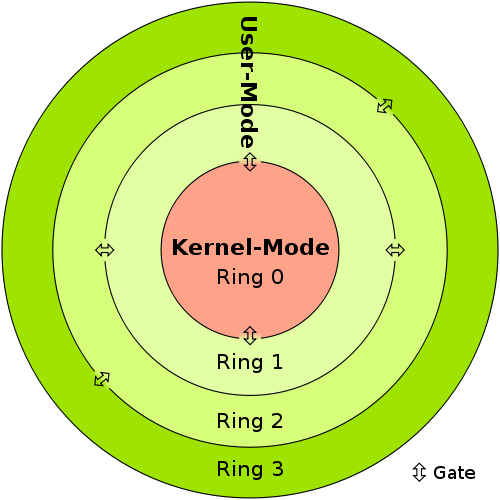
\includegraphics[width=6cm]{bilder/500px-CPU_ring_scheme.png}
    \caption{CPU Ring scheme \citep{wiki:006}}
  \end{center}
\end{figure}

Um nun mit Hilfe der Virtualisierung mehrere Betriebssysteme nebeneinander auszuführen, die sich gegenseitig nicht beeinflussen können, ist es notwendig, deren Kernel nicht im Ring 0, sondern in einem höheren Ring mit weniger Berechtigung auszuführen. Da der Programm-Code des Gast-Kernels dabei natürlich dennoch Befehle rufen würde, die nur in Ring 0 ausführbar sind, kommt es zu den eben beschriebenen Exceptions. Die Lösung dieser Ausnahmesituationen ist dabei nun Aufgabe des Hypervisors. Dazu beinhaltet ein Hypervisor immer mindestens einen Prozess, der selbst in Ring 0 läuft und in der Lage ist, die Auflösung der Ausnahmesituationen zu erledigen. Ein Hypervisor kann dabei nun verschiedene Strategien anwenden. Die einfachste Strategie ist eben, auf entsprechende Exceptions zu warten und diese zum Beispiel durch Aufrufe auf das eventuell vorhandene Host-Betriebssystem oder den Ring-0-Prozess des Hypervisors zu ersetzen. Auch wenn diese Strategie funktioniert, so ist die Behandlung tausender solcher Ausnahmesituationen sehr teuer und beinträchtigt die Leistung des Gastsystems empfindlich. Moderne Hypervisoren verfolgen deshalb eine zwar sehr viel kompliziertere aber eben auch effizientere Strategie. Sie scannen den Programm-Code des Gastsystems nach problematischen Befehlen und ersetzen diese bereits vor der Ausführung im Speicher mit Befehlen, die in der Berechtigungsstufe des Gastsystems erlaubt sind. Heutige Prozessoren kennen mitunter sogar das Konzept der Virtualisierung mittels Hypervisor und bieten spezielle Befehlssätze an, die sich besonders für diese Ersetzung eignen und sich aus eingeschränkten Berechtigungsstufen rufen lassen. Moderne Hypervisoren und Betriebssysteme kommen damit auf Ausführungszeiten, die nahezu denen auf direkter physischer Hardware entsprechen.

Die obige Beschreibung der Herausforderungen bei der Virtualisierung auf Basis der Prozessorarchitektur x86 stützen sich vor allem auf die Seiten 203-206 des Oracle VM VirtualBox User Manuals \citep{Oracle14}.

Robert P. Goldberg, der die Grundlagen des \ac{VMM} in den 70er Jahren wissenschaftlich erarbeitet hat, unterscheidet in seiner Doktorarbeit "`Architectural Principles for Virtual Computer Systems"' nun zwei Klassen des \ac{VMM} \citep[vgl.][S. 22 ff.]{Goldberg73}: Dem Typ I \ac{VMM} oder auch "`Bare Metal Hypervisor"' und dem Typ II \ac{VMM} oder auch "`Hosted Hypervisor"'. In den folgenden beiden Unterkapiteln sollen diese beiden Klassen und entsprechende Implementierungen näher beleuchtet werden.

Darauf folgt abschließend ein Unterkapitel zu den sogenannten Unikernels, einer relativ neuen Entwicklung innerhalb der Systemvirtualisierung mittels Hypervisor, die eine bestimmte Art von \ac{VM} beschreibt.

\subsubsection{Bare Metal Hypervisors}

Ein Bare Metal Hypervisor ist ein \ac{VMM}, der als eigenständiges Programm direkt auf echter physischer Hardware läuft und somit kein Betriebssystem auf dem Hostsystem benötigt.

\begin{figure}[!ht]
  \begin{center}
    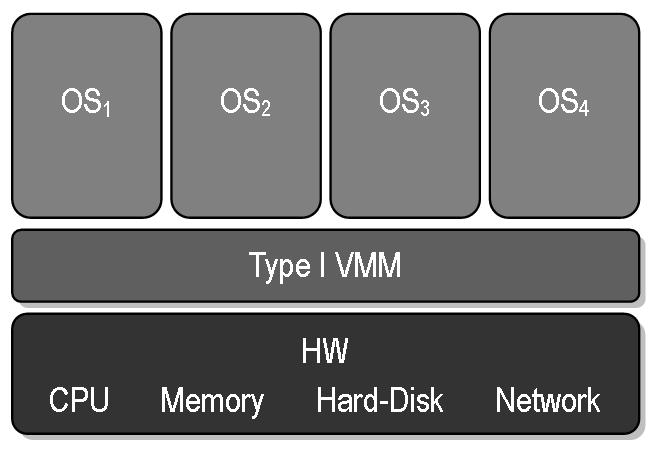
\includegraphics[width=6cm]{bilder/VMM-Type1.jpg}
    \caption{Virtual Machine Monitor Type I \citep{wiki:002}}
  \end{center}
\end{figure}

Durch diesen direkten Zugriff und das nicht notwendige Hostbetriebssystem gilt ein Bare Metal Hypervisor als ressourceneffizienter als ein Hosted Hypervisor. Größter Nachteil dieser Variante ist aber, dass sie mit mehr Installationsaufwand verbunden ist, da der Hypervisor selbst die passenden Gerätetreiber für die zugrundeliegende Hardware benötigt und man nicht auf Standardwerkzeuge wie zum Beispiel den Installationsmanagers eines Hostbetriebssystems zugreifen kann. Typische Vertreter dieser Hypervisor-Klasse sind zum Beispiel VMWare vSphere, KVM und Citrix XenServer.

\begin{figure}[!ht]
  \begin{center}
    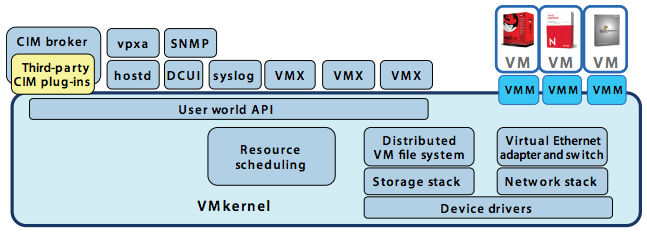
\includegraphics[width=10cm]{bilder/vmware.png}
    \caption{VMWare vSphere Architektur \citep{vmware:002}}
  \end{center}
\end{figure}

Bei VMWare vSphere handelt es sich um ein kommerzielles Produkt der Firma VMWare, dem Marktführer im Bereich der Virtualisierungslösungen mit einem Marktanteil von ungefähr 50\% \citep[vgl.][]{vmware:001}. vSphere basiert auf einem von WMWare eigens entwickelten Betriebssystem, dem sogenannten VMkernel. Auf diesem Betriebssystem laufen das Programm DCUI (Direct Console User Interface), eine Konsole zur direkten Konfiguration des Servers, und diverse weitere Schnittstellen, mit denen man die Verwaltung des Servers und der auf ihm laufenden virtuellen Maschinen auch über das Netzwerk erledigen kann. Für jede virtuelle Maschine wird ein eigener Hypervisor- und ein weiterer Hilfsprozess gestartet (VMM und VMX). vSphere bietet die Möglichkeit, virtuelle Maschinen im laufenden Betrieb von einem vSphere Server auf einen anderen zu übertragen. Diese Funktion, vMotion genannt, erleichtert das Resourcenmanagement enorm, da sich eine laufende Anwendung auf andere Hardware übertragen lässt, um die vorherige Hardware zum Beispiel zu reparieren oder auch einfach nur zur Einsparung auszuschalten.

\begin{figure}[!ht]
  \begin{center}
    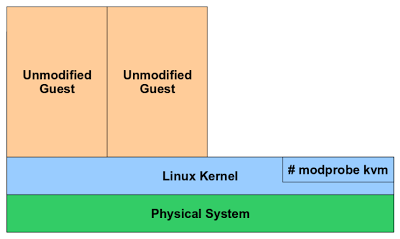
\includegraphics[width=8cm]{bilder/kvm.png}
    \caption{KVM Architektur \citep{kvm:002}}
  \end{center}
\end{figure}

Beim Open-Source-Produkt KVM (Kernel-based Virtual Machine) handelt es sich um eine Lösung, bei der ein normaler Linux-Kernel über ein spezielles Kernel-Modul für die grundsätzliche Virtualisierung (kvm.io) und ein weiteres prozessorspezifisches Kernel-Modul (kvm-intel.io oder kvm-amd.io) in die Lage versetzt wird, als Hypervisor zu arbeiten und Gastsysteme zu verwalten. KVM lässt sich damit grundsätzlich auf allen gängigen Linux Distributionen installieren. Oft wird deshalb vermutet, dass es sich nicht um einen reinen Bare Metal Hypervisor handelt, da er eben zusammen mit einem Betriebssystem installiert wird. Da es sich bei dem Kernel-Modul aber nicht um ein Anwendungsprogramm handelt, sondern um eine Erweiterung des eigentlichen Kernels, setzt diese Virtualisierungslösung direkt auf der darunterliegenden Hardware und nicht auf einem dazwischenliegenden Kernel auf \citep[Vgl.][S. 225 - 227]{KivKam07}.

So gibt es zum Beispiel die Linux Distribution Proxmox VE, die man direkt auf eine leere Hardware installieren kann und die die entsprechenden Kernel-Module und weitere Hilfsprogramme (zum Beispiel zur Verwaltung der virtuellen Maschinen) bereits beinhaltet \citep[Vgl.][]{Proxmox14}.

\begin{figure}[!ht]
  \begin{center}
    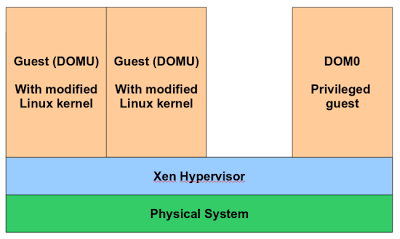
\includegraphics[width=8cm]{bilder/xen.png}
    \caption{Xen Architektur \citep{kvm:002}}
  \end{center}
\end{figure}

Auch bei XenServer von der Firma Citrix handelt es sich um ein Open-Source-Produkt. Auch dieser \ac{VMM} setzt direkt auf der eigentlichen physischen Hardware auf. XenServer basiert ebenfalls auf einem Linux-Kernel. Es handelt sich aber nicht lediglich um Kernel-Module, die sich in eine beliebige Linux-Distribution laden lassen, sondern um einen modifizerten Linux-Kernel. XenServer lässt sich also nur auf komplett leere Hardware installieren und bietet auch nicht die vollständigen Funktionalitäten einer normalen Linux-Distribution. Das besondere an XenServer ist, dass die Prozesse zur Steuerung der virtuellen Maschinen selbst in einer virtuellen Maschine laufen. Diese auch "`Privileged Guest"' genannte Maschine muss laufen, bevor weitere Gastsysteme geladen werden können. Der "`Privileged Guest"' oder auch DOM0 genannte Gast hat dabei (wie der Name sagt) besondere Rechte, die ihm die Steuerung der darunterliegenden Virtualisierungsschicht im Hypervisor ermöglichen \citep[Vgl.][S. 2]{Schee14}.

Als weitere Gastsysteme lassen sich wie auch bei KVM beliebige unmodifzierte Gastsysteme wie Linux-Distributionen oder Windows-Systeme installieren. Besonders ist aber, dass sich auch Linux-Distributionen mit ebenfalls modifiziertem Kernel laden lassen, die direkter mit dem Hypervisor zusammen arbeiten und so eine höhere Performance bieten.

\subsubsection{Hosted Hypervisors}

Ein Hosted Hypervisor ist ein \ac{VMM}, der als Anwendungsprogramm innerhalb eines Hostbetriebssystems läuft. Es ist somit möglich, auch andere Programme neben dem Hypervisor und seinen Gastbetriebssystemen zu verwenden.

\begin{figure}[!ht]
  \begin{center}
    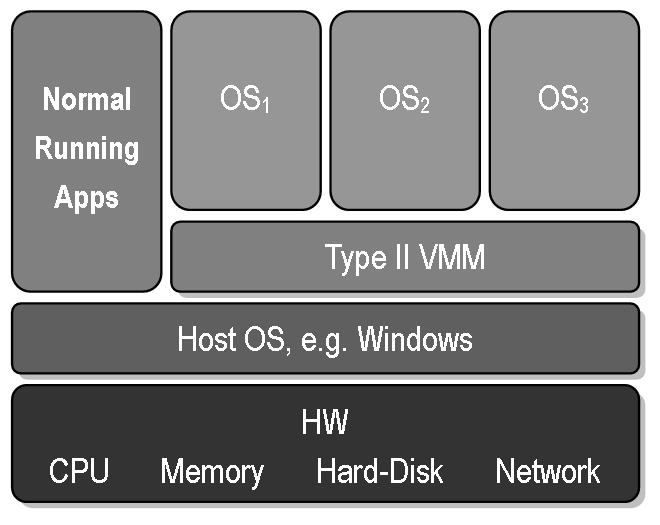
\includegraphics[width=6cm]{bilder/VMM-Type2.jpg}
    \caption{Virtual Machine Monitor Type II \citep{wiki:003}}
  \end{center}
\end{figure}

Größter Vorteil dieser Variante ist es also, dass das Hostsystem auch für gewöhnliche Benutzerarbeiten zur Verfügung steht und nicht ausschließlich zur Virtualisierung verwendet werden muss. Diese Virtualisierungslösung lässt sich sehr einfach nachträglich auf eine Vielzahl von Betriebssystemen installieren und auch wieder deinstallieren. Ein typischer Vertreter dieser Hypervisor-Klasse ist zum Beispiel VirtualBox von Oracle \citep[Vgl.][S. 24]{DamMohAnd12}.

VirtualBox bietet nach der Installation eine grafische Benutzeroberfläche, mit der man seine virtuellen Maschinen einfach verwalten kann. Zum Beispiel ist es möglich, eine neue, leere virtuelle Maschine zu definieren, ihre Hardware-Einstellungen wie zum Beispiel Menge an Prozessoren und Arbeitsspeicher zu konfigurieren und sie zu starten. Anschließend lässt sich dann zum Beispiel mit einem Installationsmedium ein Betriebssystem auf der Gast-Maschine installieren. Es lassen sich aber auch bestehende Maschinen exportieren und importieren, auf denen zum Beispiel bereits ein Betriebssystem und weitere Anwendungsprogramme installiert sind. Schließlich lassen sich virtuelle Maschinen auch einfach pausieren, stoppen und natürlich löschen \citep[Vgl.][S. 11 ff.]{Oracle14}.

\begin{figure}[!ht]
  \begin{center}
    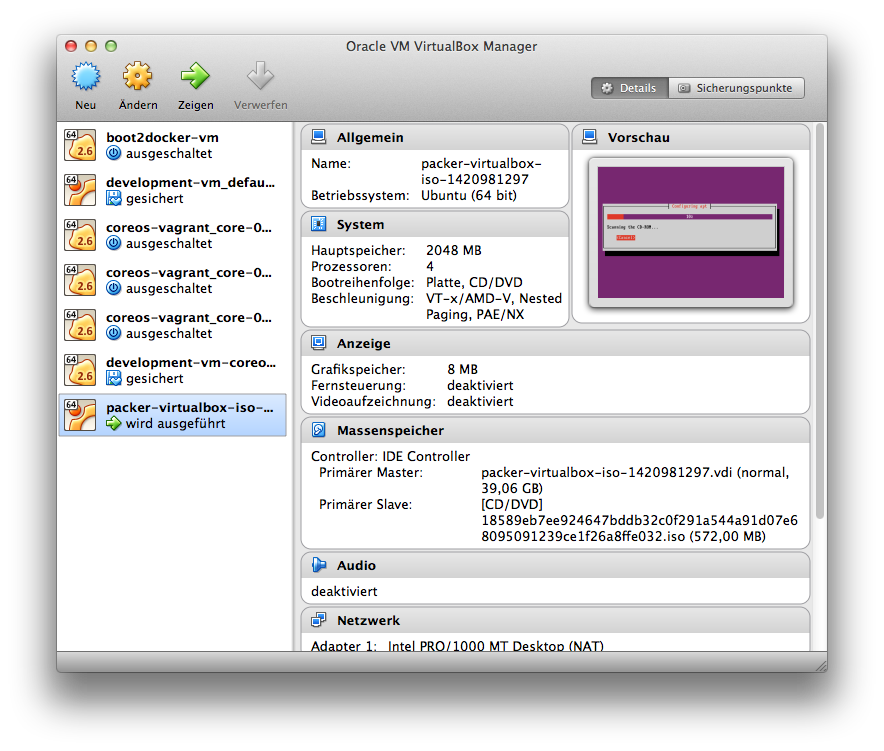
\includegraphics[width=8cm]{bilder/virtualbox-gui.png}
    \caption{Grafische Benutzeroberfläche von VirtualBox}
  \end{center}
\end{figure}

Neben der grafischen Benutzeroberfläche bietet VirtualBox aber auch alle Funktionen in Form von Kommandozeilen-Programmen an. Damit lässt sich VirtualBox auch leicht automatisiert verwenden, zum Beispiel von einem Continuous-Integration-Server aus, der Testumgebungen starten möchte \citep[Vgl.][S. 113]{Oracle14}.

\subsubsection{Unikernels}

Eine relativ neue Entwicklung innerhalb der Systemvirtualisierung mittels Hypervisor sind die sogenannten Unikernels. Vertreter dieser Idee kommen zum Beispiel aus dem Bereich der \ac{SOA} oder der Microservice Architecture. In diesen Architekturen wird versucht, die Teile eines IT-Systems als einzelne Dienste zu betrachten, die (meist über Netzwerk) miteinander kommunizieren. Es ist dabei von Vorteil, wenn diese Dienste jeweils eine bestimmte Aufgabe erledigen und über eine einfache Schnittstelle angesprochen werden können. Solche Dienste können nun jeweils über eine eigene \ac{VM} innerhalb der Virtualisierung abgebildet werden. Hierbei wird nun kritisiert, dass die Installation eines kompletten Gastbetriebssystems und die in ihm laufenden Anwendungsprogramme meist wesentlich mehr Resourcen und Programmcode verwenden und mehr Zugriffspunkte bieten, als für den eigentlichen Dienst benötigt wird. Als konzeptionelles Beispiel stellen wir uns hier einmal einen Dienst vor, der als einzige Aufgabe hat, mit Hilfe einer fortlaufenden Zahl neue Kundennummern zu generieren. Es ist nun durchaus nachvollziehbar, dass ein komplettes Gastbetriebssystem inkl. aller in ihm installierten Zubehörprogramme, Dokumentationen und Treiber sehr viel mehr Resourcen verbraucht, als für die eigentliche Operation sinnvoll erscheint. Die höhere Menge an Quellcode und typische Betriebssystemschnittstellen stellen zudem auch ein erhötes Sicherheitsrisiko dar, da sie potentiell mehr Angriffsvektoren bieten \citep[Vgl.][Abstract und Introduction]{MadMorAnd13}.

\begin{figure}[!ht]
  \begin{center}
    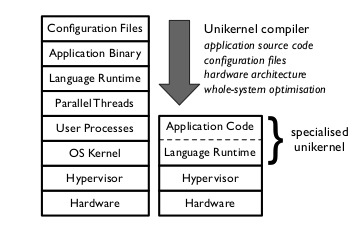
\includegraphics[width=8cm]{bilder/comparison-vm-unikernel.png}
    \caption{Vergleich klassische VM und Unikernel \citep[Abb. 1]{MadMorAnd13}}
  \end{center}
\end{figure}

Als Antwort entstehen deshalb in jüngster Vergangenheit neue Lösungen, bei denen man seinen eigentlichen Programmcode mit Hilfe einer Library entwickelt, die einfache Schnittstellen zur Verfügung stellt, um zum Beispiel Netzwerkkommunikation oder ähnliches zu betreiben. Der Programmcode wird dann mit Hilfe dieser Library in eine sehr viel kleinere \ac{VM} kompiliert, die wieder mit Hilfe eines Hypervisors ausgeführt werden kann. Ein Beispiel für eine solche Library ist MirageOS \citep[Vgl.][]{MadMorAnd13}.

Ein Nachteil dieser Lösung ist, dass man lediglich Funktionalität wiederverwenden kann, die genau durch die benutzte Library zur Verfügung steht. So kann man auch lediglich in der Programmiersprache arbeiten, die der Compiler der Library versteht. Im Falle von MirageOS ist dies die Sprache Ocaml. Es ist somit zum Beispiel nicht möglich, einen PHP-Interpreter zu starten und PHP-Scripte auszuführen, wie das mit allen gängigen Betriebssystemen wie Linux, MacOS oder Windows der Fall ist. Unikernels lassen sich somit zumindest bisher nur für sehr spezielle Dienste und Problemestellungen einsetzen.

\subsection{Betriebssystemvirtualisierung mittels OS-Containern}

Ein ganz anderer Ansatz als die Systemvirtualisierung mittels Hypervisor ist die sogenannte Betriebssystemvirtualisierung mittels OS-Container. Dabei wird nicht versucht, ein komplettes Gastsystem mit eigener, virtualisierter Hardware und eigenem Kernel auszuführen. Vielmehr basiert dieser Ansatz darauf, dass sich alle virtuellen Betriebssysteme die Hardware und einen gemeinsamen Kernel teilen. Offensichtlich lassen sich damit nicht verschiedenste Betriebssysteme auf einer Maschine virtualisieren, sondern immer nur Betriebssysteme, die auf dem gleichen Kernel basieren wie das Hostsystem. Dafür entfällt die Notwendigkeit, Hardware zu emulieren oder zu virtualisieren. In Bezug auf das Ring-Schemas des Prozessors gilt: Der gemeinsame Kernel arbeitet im Ring 0 und somit direkt auf der physischen Hardware. Das virtualisierte System beinhaltet lediglich Bibliotheken und Anwendungsprogramme und arbeitet somit in Ring 3. Die Notwendigkeit, nicht erlaubte Aufrufe zu finden und zu behandeln entfällt damit. Eine solche isolierte Umgebung, OS-Container genannt, gilt damit als grundsätzlich effizienter als komplette virtuelle Maschinen \citep[Vgl.][Introduction]{Turnball14}.

\begin{figure}[!ht]
  \begin{center}
    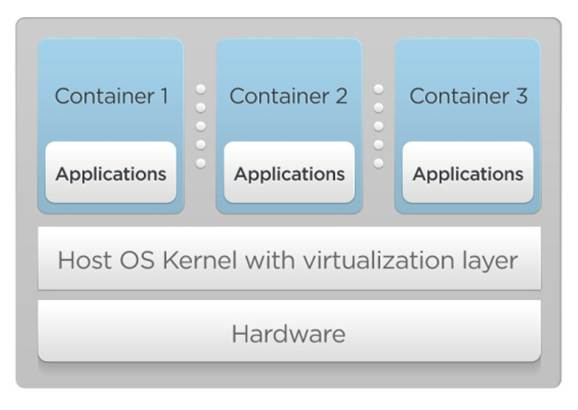
\includegraphics[width=8cm]{bilder/lxc-architecture.jpg}
    \caption{OS-Container \citep{Francis2014}}
  \end{center}
\end{figure}

Damit die einzelnen Container dennoch isoliert laufen und weder das Hostsystem noch andere Container manipulieren können, muss der Kernel spezielle Schnittstellen anbieten. Entsprechende Technologien sind im Laufe der Zeit bei einer Reihe von Betriebssystemen entwickelt worden, zum Beispiel auch für Linux und Windows. Für andere Betriebssysteme wiederum existiert keine entsprechende Schnittstelle, zum Beispiel Mac OS.

Ein prominenter Vertreter dieser Virtualisierungs-Art ist zur Zeit das Produkt Docker. Docker ist eine Open-Source-Plattform, mit deren Hilfe eine einfache Definition und Verwaltung solcher Container für den Linux-Kernel möglich ist. Kürzlich wurde aber auch eine Kooperation zwischen Microsoft und der Docker Inc., dem Unternehmen hinter Docker, bekannt gegeben. Ziel der Kooperation ist es unter anderem, dass sich entsprechende Container auch für Windows-Betriebssysteme erstellen lassen \citep[Vgl.][]{heise:001}.

Docker setzt auf eine Reihe von Schnittstellen auf, die inzwischen Teil des offizielen Linux-Kernels sind. Unter anderem gehören dazu die Cgroups und die Namespaces:

Cgroups (Control Groups) bieten die Möglichkeit, die Ressourcen-Nutzung bei der Ausführung von Prozessen durch den Kernel einzugrenzen. So lassen sich für Prozesse bestimmte Grenzen der Arbeitsspeicher- und Prozessor-Nutzung definieren. Außerdem lassen sich solche Prozesse auch komplett stoppen beziehungsweise pausieren und wieder starten \citep[Vgl.][S. 3]{Schee14}.

Kernel Namespaces erlauben es, die Sichtbarkeit von Prozessen untereinander einzugrenzen. So können über Namespaces zum Beispiel die Prozess-Identifikatoren (PIDs) für jeden Container neu vergeben werden. Jeder Container kann somit einen Prozess mit der ID 1 besitzen. Aber auch andere Aspekte des Betriebssystems, wie zum Beispiel Hostname, Benutzer-IDs, Dateisystem und Netzwerk-Zugriffe lassen sich mit den Kernel Namespaces voneinander trennen \citep[Vgl.][S. 3]{Schee14}.

Docker bietet zusätzlich ein weiteres nützliches Feature, sogenannte Union-Filesystems:

\begin{figure}[!ht]
  \begin{center}
    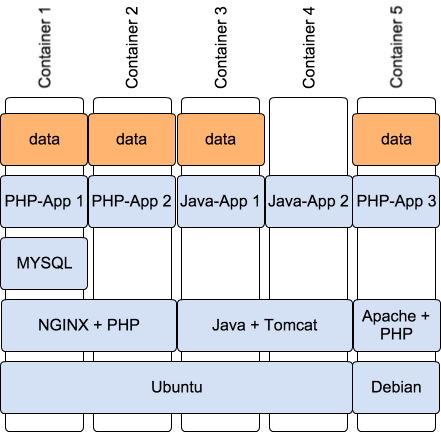
\includegraphics[width=8cm]{bilder/UnionFilesystem.png}
    \caption{Union Filesystem}
    \label{Union Filesystem}
  \end{center}
\end{figure}

Union-Filesystems sind Dateisysteme, die es erlauben, Dateisysteme transparent übereinander zu legen, um so weniger Speicherplatz zu verbrauchen. Das zugrundeliegende Verfahren nennt sich Copy-On-Write. Verwenden zwei Container zum Beispiel die gleiche Linux-Distrubution, so werden die entsprechenden Libraries und Anwendungsprogramme nur einmal auf der Festplatte vorgehalten. Das entsprechende Dateisystem wird dabei read-only unter ein für den Container beschreibbares Dateisystem gelegt. Die beiden Container unterscheiden sich also auf der Festplatte nur durch die tatsächlich individuell von ihnen geschriebenen Daten. Die meisten Union-Filesysteme erlauben dabei ein mehrfaches Übereinanderlegen, so dass eine ganze Hierarchie an ineinander verschachtelten Dateisystemen entstehen kann, um die Unterschiede zwischen den einzelnen Containern maximal effizient auf der Festplatte abzulegen \citep[Vgl.][S. 3]{Schee14}.

In der Abbildung \ref{Union Filesystem} wird zum Beispiel die gesamte Ubuntu-Distribution nur einmal auf der Festplatte abgelegt, obwohl sie von vier laufenden Containern verwendet wird. Sämtliche Dateisysteme sind read-only, bis auf die in rot angedeuteten Kästen, in denen die Container Laufzeitdaten speichern. Container 4 schreibt aber zum Beispiel keine Daten und ist somit komplett nur lesend.

\subsection{Vergleich der Virtualisierungsansätze}

TODO

\section{Konzeption zweier konkreter Lösungen}

Im Folgenden sollen nun zwei konkrete Lösungen zur Erzeugung von Test- bzw. Betriebsumgebungen skizziert werden. Die konkret verwendeten Virtualisierungslösungen werden dabei von der Pixelhouse GmbH vorgegeben.

Zum einen setzt die Pixelhouse GmbH bereits Oracles VirtualBox ein, um eine lokale Entwicklungsumgebung für die Anwendung der Webseite chefkoch.de auf den Laptops der Entwickler vorzuhalten. VirtualBox ist somit bereits auf fast allen Rechnern vorhanden und es existieren grundlegende Kenntnisse und Erfahrungen für dieses Produkt.

Zum anderen wird aktuell von Seiten der Server-Administratoren das Produkt Docker eingeführt, um die Produktivumgebung der Plattform zu betreiben. Diverse Produktiv-Komponenten der Webseite chefkoch.de laufen also bereits innerhalb von Linux-Containern. Die ersten Erfahrungen der Administratoren sind dabei vielversprechend. Es besteht der Wunsch, Probleme zu minimieren, die auftreten, weil Entwicklungs-, Test- und Produktivumgebungen nicht die gleiche Technologie verwenden und sich so grundlegend voneinander unterscheiden.

Nachfolgend soll nun zunächst die aktuelle Produktiv- und die aktuellen Testumgebungen beschrieben werden. Anschließend soll eine Betriebsumgebung definiert werden, die im Rahmen dieser Arbeit die Lösbarkeit der bisherigen Probleme mit Hilfe der Virtualisierungstechnologien zeigen kann. Zudem sollen die eingangs in der Problemstellung angedeuteten Probleme bei der Ausführung von Tests genauer erläutert und durch stark eine vereinfachte Anwendung inklusive entsprechend vereinfachter Tests dargestellt werden. Anschließend kann dann für die beiden Produkte VirtualBox und Docker ein Konzept erarbeitet werden, wie sich diese Umgebung mit Hilfe der entsprechenden Technologie virtualisieren lässt, um damit die zuvor definierte Anwendung und ihre Tests erfolgreich auszuführen.

\subsection{Beschreibung der aktuellen Produktivumgebung}

Die Betriebsumgebung die von der Pixelhouse GmbH in Produktion eingesetzt wird und täglich mehrere Millionen Anfragen von Besuchern der Webseite chefkoch.de beantwortet, besteht aus einer Vielzahl von Komponenten und Diensten. Bis auf die unternehmensweite Groupwarelösung (E-Mails, Kalender, etc.), die bereits als Dienste in Docker-Containern virtualisert werden, handelt es sich dabei um echte Maschinen, die jeweils auf ihrer eigenen Hardware laufen.

\begin{figure}[!ht]
  \begin{center}
    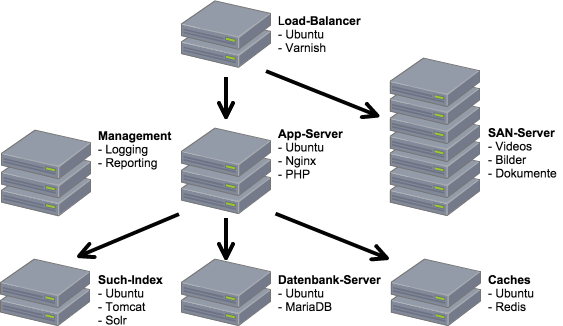
\includegraphics[width=10cm]{bilder/Produktiv-Umgebung.png}
    \caption{Die Produktiv-Umgebung der Webseite chefkoch.de}
  \end{center}
\end{figure}

Im Zentrum der Infrastruktur stehen insgesamt drei Appserver. Bei jedem Appserver handelt es sich dabei um einen Ubuntu-Server, auf dem der Webserver Nginx und der Script-Interpreter PHP ausgeführt wird, um HTTP-Anfragen mit Hilfe statischer oder dynamische Inhalte zu beantworten. Für die langfristige Datenhaltung greifen die PHP-Scripte dabei auf zwei Datenbankserver (Master und Slave) zu, auf denen ebenfalls Ubuntu und der Mysql-Fork MariaDB installiert sind. Für kurzfristige und hochverfügbare Datencaches gibt es zwei Ubuntu-Server (Master und Slave) auf denen der Key-Value-Store Redis läuft. Zudem wird auf weiteren zwei Ubuntu-Servern (Master und Slave) ein Such-Index mit Hilfe der Suchmaschine Solr betrieben, die als Java-Anwendung in einem Tomcat-Application-Server läuft. Binärdateien (Videos, Bilder, Dokumente, etc.) werden auf insgesamt 7 weiteren Servern redundant abgelegt. Damit die Appserver und die SAN-Server von außen unter einheitlichen HTTP-Adressen erreichbar sind und sich die Last gleichmäßig auf die einzelnen Server verteilt, landen sämtliche HTTP-Anfragen per DNS-Round-Robin zunächst bei einem von zwei Ubuntu-Servern, auf denen Varnish als Load-Balancer installiert ist. Diese nehmen die Anfragen entgegen und verteilen sie an die dahinter liegenden Server. Varnish ist zudem ein effizienter HTTP-Cache, der in der Lage ist, die von den App- oder SAN-Servern zurückgelieferten Antworten zu cachen und bei erneuter Anfrage selbst auszuliefern. Zu guter Letzt gibt es noch drei weitere Server, auf denen Software für die Administration und das Reporting läuft.

\subsection{Beschreibung der aktuellen Testumgebungen}

Die aktuellen Testumgebungen der Pixelhouse GmbH besitzen einen extrem reduzierten Aufbau. Die Testumgebungen werden alle auf ein und der selben Hardware-Maschine installiert. Fast alle Komponenten der zuvor beschriebenen Produktiv-Umgebung werden dabei von den einzelnen Testumgebungen gemeinsam verwendet. Beispielsweise nutzen alle Testumgebungen den gleichen Varnish für Load-Balancing und Caching. Dieser reicht die HTTP-Anfragen an den selben Nginx-Web-Server und PHP-Interpreter weiter und cached die Antworten bei Bedarf gleichermaßen. Als Backend-Dienste werden die selbe MariaDB-Datenbank, der selbe Redis-Cache und der selbe Solr-Such-Index verwendet. Die Binärdateien werden ebenfalls auf dem selben Host von allen Testumgebungen gemeinsam verwendet. Einziger Unterschied zwischen den einzelnen Testumgebungen ist, dass aufgrund einer speziellen Konfiguration im Nginx-Webserver je nach aufgerufener URL vom PHP-Interpreter andere PHP-Scripte geladen werden und somit jeweils eine andere Version der PHP-Anwendung getestet werden kann.

\begin{figure}[!ht]
  \begin{center}
    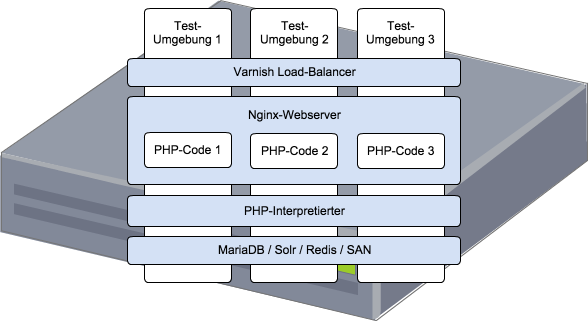
\includegraphics[width=10cm]{bilder/Aktuelle-Testumgebung.png}
    \caption{Die aktuelle Test-Umgebung}
  \end{center}
\end{figure}

Die aktuelle Testumgebung bringt Probleme in Bezug auf die Testbarkeit der Anwendung mit sich. Da alle Testumgebungen zum Beispiel die gleichen Backend-Dienste verwenden, ist es mitunter nicht möglich, die für den Test notwendigen Testdaten zu erzeugen, ohne damit Einfluss auf andere Testumgebungen zu nehmen. Ein weiteres Problem ist, dass nur Änderungen am PHP-Code selbst testbar sind. Will man zum Beispiel eine Änderung am HTTP-Caching im Varnish testen, kann man diese nur in allen Testumgebungen gleichermaßen vornehmen.

\subsection{Definition einer verifizierbaren Testumgebung}

Um nun eine zwar möglichst leicht zu implementierende, für die Darstellung der Lösbarkeit dieser Probleme aber hinreichende Umgebung zu definieren, werden folgende Änderungen vorgenommen:
Zunächst wird die Anzahl gleicher Komponenten auf jeweils eins reduziert. Außerdem werden die Caches und der Such-Index ausgeblendet, da sie genau wie die Datenbankserver aus den Appserver heraus als Backend-Dienst abgefragt werden und lediglich eine andere Technologie beziehungsweise einen anderen Schwerpunkt der Datenhaltung widerspiegeln (Kurzfristigkeit und Durchsuchbarkeit). Zuletzt ignorieren wir im Rahmen dieser Arbeit die SAN- und Management-Server.

\begin{figure}[!ht]
  \begin{center}
    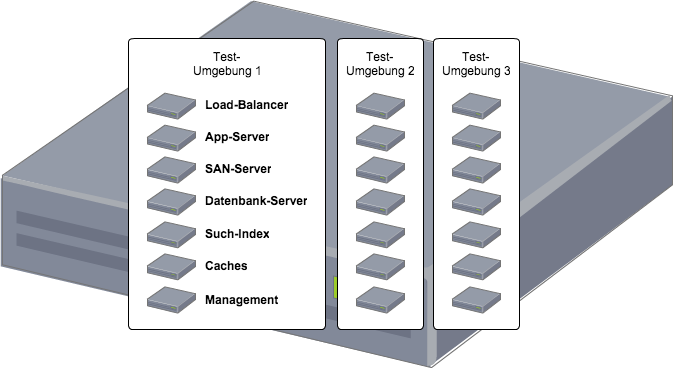
\includegraphics[width=4cm]{bilder/Untersuchungs-Umgebung.png}
    \caption{Für die Untersuchung definierte Umgebung}
  \end{center}
\end{figure}

Die von uns definierte Umgebung besteht somit lediglich aus einem Varnish-Load-Balancer, einem Nginx-Appserver, der den Script-Interpreter PHP ausführt und einen Maria-DB-Server, der aus PHP heraus als Backend-Dienst abgefragt werden kann.

\subsection{Definition von Anwendungs- und Testfällen}

Für die Verifizierung der jeweiligen Testumgebungen ist es notwendig, eine andere PHP-Anwendung als die echte Anwendung der Webseite chefkoch.de zu verwenden. Zum einen ist die echte PHP-Anwendung auf dieser reduzierten Testumgebung nicht lauffähig. Zum anderen hat sie im Laufe der Jahre eine Komplexität erreicht, die es schwer macht, einen einfachen Anwendungsfall zu finden, der dennoch die Notwendigkeit von isolierten Testumgebungen aufzeigt.

Es ist deshalb von Vorteil im Rahmen dieser Arbeit neue PHP-Scripte mit einzelnen Anwendungsfällen zu definieren, die die zuvor angedeuteten Probleme beim Ausführen der Tests, die auf eine mangelnde Isolation einzelner Test-Umgebungen zurückzuführen sind, einfach provozieren. Passend dazu lassen sich dann ebenso einfache Testfälle definieren, die zeigen, ob die neue Testumgebungen mit Hilfe der Virtualisierungstechnologien die eingangs erläuterten Probleme einfach lösen.

\subsubsection{Isolierte Testdaten in der Datenbank}

Wir denken uns einen einfachen Anwendungsfall aus, der Daten derart in die Datenbank schreibt, dass es Einfluß auf andere Testumgebungen haben würde, wenn sich mehrere Testumgebungen die gleiche Datenbank teilen. Dazu reicht es zum Beispiel aus, einen einfachen Zähler zu implementieren. Dieser Zähler legt zunächst, falls noch nicht vorhanden, eine neue Tabelle an, die eine Integer-Spalte enthält und fügt einen Datensatz mit dem Wert 0 ein. Falls die Tabelle schon existiert, erhöht er den Wert um eins. Der aktuelle Wert wird anschließend ausgegeben. Dieser Anwendungsfall sollte also beim ersten Aufruf eine 0 ausgeben und bei jedem weiteren Aufruf einen um eins erhöhten Wert (1, 2, 3, 4...).

Zum Test der Testdaten-Isolierung muss man nun lediglich zwei Testumgebungen anlegen und sicherstellen, dass beide Umgebungen unabhängig voneinander zählen.

\subsubsection{Konfigurationsänderung im HTTP-Cache}

Um eine Änderung am HTTP-Caching zu testen, brauchen wir zunächst ein einfaches PHP-Script, das zum einen die aktuelle Uhrzeit ausgibt und zum anderen einen HTTP-Cache-Header mitsendet, der HTTP-Caches dazu veranlasst, die HTTP-Antwort für 10 Sekunden zu cachen.
Es ist nun per Varnish-Konfiguration möglich, diese HTTP-Header für bestimmte URLs zu berücksichtigen oder eben nicht.

Damit sollte es möglich sein, eine Testumgebung zu starten, die beim Aufruf des PHP-Scriptes immer die aktuelle Uhrzeit anzeigt. Gleichzeitig muss es möglich sein, eine weitere Testumgebung zu starten, in der das gleiche HTTP-Cache nur alle 10 Sekunden die aktuelle Uhrzeit anzeigt.

\subsection{VirtualBox}

\subsection{Docker}

\section{Implementierung}

Bei der prototypischen Implementierung der zuvor konzipierten Testumgebung mit Hilfe des Hosted-Hypervisor Oracle VirtualBox und der OS-Containervirtualisierung Docker konnten sowohl Gemeinsamkeiten als auch Unterschiede in den beiden Ansätzen festgestellt werden.

Grundsätzlich beiden Ansätzen gemeinsam ist, dass zunächst ein ausführbares Abbild der einzelnen Komponenten erzeugt werden muss. Anschließend braucht es jeweils eine Möglichkeit, die so entstandenen Abbilder zusammen zur Ausführung zu bringen und ihnen eine Kommunikation untereinander zu ermöglichen.

Wie nun im Folgenden beschrieben wird, unterscheiden sich die beiden Ansätze dabei vor allem in der Einfachheit, die einzelnen Komponenten als gemeinesame Umgebung zu definieren und zu starten.

Die vollständige Implementierung beider Ansätze kann übrigens der beigefügten CD entnommen oder unter folgender Adresse online eingesehen werden:

\href{https://github.com/perprogramming/bachelor-arbeit/tree/master/cd/Implementierung}{https://github.com/perprogramming/bachelor-arbeit/tree/master/cd/Implementierung}

\subsection{VirtualBox}

Um die zuvor konzipierte Testumgebung mit VirtualBox zu virtualisieren, ist es zunächst notwendig, fertige virtuelle Maschinen zu erzeugen, die sich bei Bedarf direkt mit VirtualBox starten lassen. Ein Werkzeug zur Erzeugung solcher Maschinenabbilder ist Packer \citep[Vgl.][]{Packer15}.

Es wäre außerdem von Vorteil, das Starten der einzelnen Maschinen nicht selbstständig steuern zu müssen. Ein Werkzeug, mit dem man mehrere virtuelle Maschinen zu einer Gesamtumgebung auf Basis von VirtualBox orchestrieren kann, ist Vagrant \citep[Vgl.][]{Vagrant:001}.

Im Folgenden wird nun die Funktionsweise der beiden Werkzeuge Packer und Vagrant genauer beschrieben.

\subsubsection{Erzeugung der einzelnen Maschinen mit Packer}

"`Packer is a tool for creating identical machine images for multiple platforms from a single source configuration."' \citep[S.][]{Packer15} Packer kennt dabei vor allem drei wichtige Konzepte: Builder \citep[Vgl.][]{Packer:001}, Provisioner \citep[Vgl.][]{Packer:002} und Post-Processor \citep[Vgl.][]{Packer:003}. Diese werden mit Hilfe der Konfigurations-Datei namens packer.json definiert. Die Abbildung \ref{Loadbalancer-Packer} zeigt die entsprechende Konfigurations-Datei für die Komponente des Loadbalancers.

\begin{figure}[!ht]
  \begin{center}
    \externalcode{json}{cd/Implementierung/machines/loadbalancer/packer.json}
    \caption{packer.json für den Loadbalancer}
    \label{Loadbalancer-Packer}
  \end{center}
\end{figure}

Ein Builder \citep[Vgl.][]{Packer:001} beschreibt eine bestimmte Technologie, mit deren Hilfe das virtuelle Maschinen-Abbild erzeugt wird. Neben verschiedenen anderen Technologien beinhaltet Packer auch Builder zur Erzeugung von virtuellen Maschinen mit VirtualBox. Grundsätzlich gibt es dabei zwei Möglichkeiten: Zum einen kann man einen Builder vom Typ "`virtualbox-iso"' verwenden. Mit diesem wird eine leere virtuelle Maschine erzeugt und anschließend mit Hilfe eines Installationsmedium im ISO-Format (\acl{ISO}) ein Betriebssystem installiert. Zum anderen kann man einen Builder vom Typ "`virtualbox-ovf"' verwenden. Das Format OVF (\acl{OVF}) ist ein generisches Format zum Import und Export von virtuellen Maschinen. Mit diesem Builder kann man also mit Hilfe von Packer ein Maschinen-Abbild auf Basis eines anderen Maschinen-Abbildes erzeugen. So kann man zum Beispiel eine fertig installierte Linux-Distribution als Ausgangspunkt zur Installation weiterer Anwendungsprogramme verwenden. Für die Testumgebung der Pixelhouse GmbH sollen die einzelnen virtuellen Maschinen idealerweise auf Basis einer fertigen Installation von Ubuntu 14.04 Server erzeugt werden, die auch im Produktivbetrieb zum Einsatz kommt.

Um nun weitere Software auf der mit dem Builder erzeugten virtuellen Maschine zu installieren, kommt ein sogenannter Provisioner \citep[Vgl.][]{Packer:002} zum Einsatz. Ein Provisioner ist für Packer eine Technologie, mit der es einfach möglich ist, solche Installationsvorgänge zu konfigurieren. Dabei gibt es sehr umfangreiche Ansätze wie die Werkzeuge Puppet \citep[][]{puppet} oder Chef \citep[][]{chef}, die sehr mächtige Konfigurationssprachen bieten, um verschiedenste Installations- und Konfigurationsschritte in einem Betriebssystem vorzunehmen. Eine andere, eher einfache Variante wäre aber zum Beispiel der Provisioner vom Typ "`shell"', bei dem eben lediglich ein Shell Script innerhalb der virtuellen Maschine ausgeführt wird, um weitere Einstellungen oder Installationen vorzunehmen. Die Abbildung \ref{Loadbalancer-Install} zeigt zum Beispiel das entsprechende Script für den Loadbalancer. Ein Vorteil solcher Scripte ist, dass sie sich später auch sehr leicht für die Implementierung mit Hilfe von Docker wiederverwenden lassen.

\begin{figure}[!ht]
  \begin{center}
    \externalcode{bash}{cd/Implementierung/machines/loadbalancer/contents/install.sh}
    \caption{Provisionierungs-Script für den Loadbalancer}
    \label{Loadbalancer-Install}
  \end{center}
\end{figure}

Schließlich kennt Packer nun noch das Konzept des Post-Prozessors \citep[Vgl.][]{Packer:003}. Ein Post-Prozessor meint dabei eine bestimmte Art und Weise, mit der das fertige Maschinen-Abbild exportiert und für die Verwendung mit anderen Tools vorbereitet wird. So gibt es eben einen Post-Prozessor vom Typ "`Vagrant"', der es ermöglicht, das fertige Maschinen-Abbild direkt mit Vagrant innerhalb einer Testumgebung zu starten. Damit sollte es möglich sein, die einzelnen fertigen virtuellen Maschinen der Testumgebung so abzulegen, dass man sie sofort als Gesamtumgebung starten kann.

\subsubsection{Umgebungssteuerung mit Vagrant}

"`Vagrant provides easy to configure, reproducible, and portable work environments built on top of industry-standard technology and controlled by a single consistent workflow [..]."' \citep[S.][]{Vagrant:001} Vagrant vermittelt also zwischen anderen Werkzeugen, um einen einfachen Einstiegspunkt zum Starten einer Umgebung zu bieten.

\begin{figure}[!ht]
  \begin{center}
    \begin{rubycode}
Vagrant.configure(2) do |config|
    cwd = File.dirname(__FILE__)
    ...
    config.vm.define "app" do |app|
        app.vm.box = "app"
        app.vm.box_url = "file://" + cwd + "/machines/app/vagrant.box"
        app.vm.hostname = "app"
        app.vm.network "private_network", ip: "172.28.128.6"
        app.ssh.password = "vagrant"
        app.ssh.insert_key = false
        app.vm.provider "virtualbox" do |v|
            v.memory = 256
            v.cpus = 1
        end
        app.vm.provision "hosts"
    end
    
    config.vm.define "loadbalancer" do |loadbalancer|
        loadbalancer.vm.box = "loadbalancer"     
        loadbalancer.vm.box_url = "file://"
            + cwd + "/machines/loadbalancer/vagrant.box"
        loadbalancer.vm.hostname = "loadbalancer"
        loadbalancer.vm.network "private_network", ip: "172.28.128.7"
        loadbalancer.vm.network "forwarded_port", guest: 80, host: 8080
        loadbalancer.ssh.password = "vagrant"
        loadbalancer.ssh.insert_key = false
        loadbalancer.vm.provider "virtualbox" do |v|
            v.memory = 256
            v.cpus = 1
        end
        loadbalancer.vm.provision "hosts"
        loadbalancer.vm.provision "shell",
            inline: "sudo service varnish start",
            keep_color: true
    end
end
    \end{rubycode}
    \caption{Auszug aus der Vagrantfile der neuen Testumgebung}
    \label{Vagrantfile}
  \end{center}
\end{figure}

Dazu legt man zunächst eine Konfigurationsdatei namens Vagrantfile an, in der man seine Umgebung definiert. Vagrant bietet dabei die Möglichkeit, eine oder mehrere virtuelle Maschinen auf Basis von verschiedenen Virtualisierungstechnologien zu starten. So bietet es eben auch die Möglichkeit, virtuelle Maschinen mit Hilfe von VirtualBox zu starten, die mit Packer vorbereitet wurden. Es bietet weiterhin einfache Konfigurationsparameter, die zum Beispiel die Netzwerkkommunikation zwischen den virtuellen Maschinen und dem Host-Betriebssystem und auch untereinander ermöglichen. Auch einzelne Parameter wie Anzahl der virtuellen Prozessoren und die Menge des zur Verfügung gestellten Arbeitsspeicher lassen sich hier noch nachträglich definieren. Es ist auch möglich, Ordner zwischen dem Host-Betriebssystem und den virtuellen Maschinen zu teilen, um so zum Beispiel während der Entwicklung mit einer IDE (\acl{IDE}) auf dem Host-Betriebssystem Code zu bearbeiten, der direkt in den virtuellen Maschinen ausgeführt wird. Es ist also möglich, eine mit Vagrant betriebene Umgebung nicht nur zu Testzwecken sondern auch für die lokale Entwicklung auf einem Entwickler-Laptop zu verwenden.

Die Abbildung \ref{Vagrantfile} zeigt einen Auszug aus der fertigen Konfigurationsdatei. Eine Besonderheit ist hier durch die Einstellung \textit{loadbalancer.vm.provision "`hosts"'} gegeben. Um nämlich die Kommunikation der einzelnen Komponenten untereinander zu ermöglichen, wird das Vagrant-Plugin "`vagrant-hosts"' \citep[Vgl.][]{vagranthosts} verwendet. Dieses wird über diese Konfigurationszeile dazu veranlasst, in die Datei \textit{/etc/hosts} jeder Komponente statische IP-Einträge (\acl{IP}-Einträge) auf die anderen Komponenten einzutragen. So kann zum Beispiel der Appserver davon ausgehen, dass er den Datenbankserver einfach unter dem Hostnamen \textit{database} findet. Ein Nachteil dieser Lösung ist aber, dass die Provisionierung erst stattfindet, nachdem das Betriebssystem und alle installierten Dienste gestartet wurden. Da Varnish nicht korrekt startet, solange er die IP-Adressen seiner Backends (in diesem Fall die Maschine des Appservers) auflösen kann, muss ein erneutes Starten veranlasst werden, nachdem das Plugin "`vagrant-hosts"' die Adresse der Appserver-Komponente eingetragen hat. Deshalb sieht man in der Konfigurationsdatei danach noch einen weiteren Provider, der den Varnish-Service erneut startet. In der Abbildung \ref{varnishconf} ist die entsprechende Konfiguration des Backends in Varnish zu sehen.

\begin{figure}[!ht]
  \begin{center}
    \begin{yamlcode}
backend default {
    .host = "app";
    .port = "80";
}
    \end{yamlcode}
    \caption{Auszug aus der Konfigurationsdatei von Varnish}
    \label{varnishconf}
  \end{center}
\end{figure}

Mit Hilfe der fertigen Konfigurationsdatei lässt sich nun die entsprechende Umgebung mit einem einfach Kommandozeilen-Befehl starten: "`vagrant up"'. Vagrant lädt und startet dann alle in der Konfigurationsdatei angegebenen Maschinen und setzt die gewünschten Konfigurationen für Netzwerkkommunikation und Hardware-Parameter um.

Anschließend lässt sich die innerhalb der Umgebung laufende Anwendung zum Beispiel mit einem Browser des Host-Betriebssystems ansteuern.

Wie im Kapitel Grundlagen beschrieben, kann es beim Durchführen von Integrationstests vorteilhaft sein kann, nur Teile der gesamten Umgebung zu starten. So kann es zum Beispiel Integrationstests geben, die lediglich das Zusammenspiel von einzelnen Klassen der Anwendung mit der Datenbank testen. Vagrant bietet deshalb die Möglichkeit, gezielt auch nur einzelne Komponenten zu starten oder auch zu stoppen. Dazu kann man dem entsprechenden Befehl einfach die Namen der zu steuernden Komponenten übergeben, zum Beispiel "`vagrant up app database"'.

\subsection{Docker}

Auch bei der Verwendung von Docker zur Virtualisierung der Testumgebung mit Hilfe von OS-Containern stellt sich zunächst die Frage, wie man die einzelnen Container erzeugt. Im Gegensatz zu VirtualBox ist dazu keine weitere Software notwendig, da Docker bereits selbst die Möglichkeit zur Erzeugung solcher Images mit sich bringt. Es ist dazu lediglich notwendig, eine einfach Definitionsdatei, eine sogenannte Dockerfile, zu schreiben \citep[Vgl.][]{docker:003}.

Eine Möglichkeit zur Orchestrierung der einzelnen Container zu einer Gesamtumgebung wird ebenfalls von der Docker Inc. angeboten und nennt sich docker-compose \citep[Vgl.][]{dockercompose}.

Sowohl auf die Verwendung der Dockerfiles als auch auf die Verwendung von docker-compose wird im Folgenden näher eingegangen.

\subsubsection{Images mit Dockerfiles bauen}

Docker bietet eine einfache, integrierte Möglichkeit, neue Maschinen-Abbilder zu erzeugen \citep[Vgl.][]{docker:003}. Wie im Grundlagen-Kapitel beschrieben, werden diese Maschinen-Abbilder mit Hilfe eines Union-Filesystems gestartet. Einzelne Abbilder lassen sich so durch das Hinzufügen eines weiteren, überlagernden Dateisystems zu neuen Abbildern erweitern. Die Definitions-Datei eines Docker-Images, Dockerfile genannt, startet deshalb immer mit der Angabe des zugrundeliegenden Images. Anschließend lassen sich einfach Kommandozeilen-Befehle definieren, die in der laufenden Maschine ausgeführt werden. Führen diese Befehle zu Änderungen am Dateisystem, so werden diese Änderungen eben in einer neuen Dateisysteme-Ebene festgehalten, die Teil des fertigen Abbildes wird. Genauso einfach lassen sich auch Dateien in die Maschine kopieren, die auf dem Host-System liegen. Schließlich lässt sich auch ein Befehl konfigurieren, der standardmäßig ausgeführt wird, wenn man das Image später als Container startet. Die Abbildung \ref{loadbalancer-dockerfile} zeigt die entsprechende Datei für die Loadbalancer-Komponente. Hier ist nun zu sehen, dass wir das gleiche Installations-Script wie bei der Erzeugung der Maschinen-Abbilder für VirtualBox verwenden können.

\begin{figure}[!ht]
  \begin{center}
    \externalcode{docker}{cd/Implementierung/machines/loadbalancer/Dockerfile}    
    \caption{Dockerfile des Loadbalancers}
    \label{loadbalancer-dockerfile}
  \end{center}
\end{figure}

Ein Image lässt sich dann einfach mit dem Befehl "`docker build -t chefkoch/loadbalancer ."' erzeugen. Anschließend lässt sich das Image mit dem Befehl "`docker run chefkoch/loadbalancer"' als Container ausführen. Es ist sogar möglich, das fertige Image mit dem einfachen Befehl "`docker push chefkoch/loadbalancer"' in einem Web-Verzeichnis, der sogenannten docker-registry unter \href{https://registry.hub.docker.com/}{https://registry.hub.docker.com/}, zu veröffentlichen \citep[Vgl][]{docker:004}. So ist es jedem möglich, dieses Image oder auch andere Images des Verzeichnisses als Basis für ein weiteres Image zu verwenden oder auch einfach nur als Container auszuführen. Solange die Container aber auf dem selben Hardware-Host erzeugt und gestartet werden, benötigt man diese Funktionalität nicht.

Eine praktische Eigenschaft des Build-Vorgangs von docker ist, dass er sich die Stände des Builds zwischen den einzelnen Anweisungen merkt. Wird also mitten in einer Dockerfile eine Änderung vorgenommen, so werden nur die Anweisungen ab der Änderung erneut ausgeführt, da das Ergebnis bis zu der geänderten Anweisung noch vorliegt. Besonders wertvoll ist diese Funktionalität, wenn der Build des Images zum Beispiel durch einen CI-Server regelmäßig ausgeführt wird, obwohl sich an der Dockerfile garnichts geändert hat. In diesem Falle würde der Build sofort fertig sein, da sich Docker das letzte Ergebnis gemerkt hat.

\subsubsection{Steuerung der Umgebung mit docker-compose}

Um nun die mit Docker erzeugten Images zu einer Gesamtumgebung zu orchestrieren, bietet sich das Tool docker-compose \citep[Vgl.][]{dockercompose} an. Dieses kümmert sich darum, einzelne Komponenten mit Hilfe der Anwendung docker zu starten. Dafür muss zunächst eine Konfigurationsdatei namens docker-compose.yml definiert werden, in der die einzelnen Maschinen der Umgebung und weitere Einstellungen wie zum Beispiel zur Netzwerkkommunikation zwischen den Maschinen konfiguriert werden. Die Abbildung \ref{dockercomposeyml} zeigt die fertige Konfigurationsdatei für die neue Testumgebung.

\begin{figure}[!ht]
  \begin{center}
    \externalcode{yaml}{cd/Implementierung/docker-compose.yml}
    \caption{Die docker-compose.yml der neuen Testumgebung}
    \label{dockercomposeyml}
  \end{center}
\end{figure}

Auch bei diesem Ansatz müssen die einzelnen Komponenten in der Lage sein, miteinander zu kommunizieren. Tatsächlich geschieht dies ebenfalls dadurch, dass in die Datei "`/etc/hosts"' der einzelnen Komponenten statische IP-Einträge auf anderen Komponenten eingetragen werden. Tatsächlich ist dazu aber kein zusätzliche Plugin wie bei Vagrant notwendig, da docker-compose selbst eine entsprechende Funktionalität mitbringt, die sogenannten Container-Links \citep[Vgl.][]{dockerlinks}. Wie in der Abbildung \ref{dockercomposeyml} zu sehen, kann man an eine konkrete Komponte einfach Links zu anderen Komponenten eintragen. So kann auch hier der Appserver einfach unter dem Hostnamen \textit{database} auf den Datenbankserver zugreifen. Diese Verlinkung wird bereits vor dem Starten des eigentlichen Containers und seiner Prozesse umgesetzt, so dass kein erneutes Starten des Loadbalancers wie bei der Lösung mit VirtualBox beziehungsweise Vagrant notwendig ist.

Die neue Testumgebung lässt sich schließlich mit dem einfachen Befehl "`docker-compose up"' starten.

Auch docker-compose bietet die Möglichkeit, für das Durchführen von Integrationstests nur Teile der gesamten Umgebung zu starten. Dazu kann man dem entsprechenden Befehl einfach die Namen der zu jeweiligen Komponenten übergeben, zum Beispiel "`docker-compose up app database"'. Dabei berücksichtigt docker-compose allerdings die Verlinkung der einzelnen Komponenten. Da die Appserver-Komponente, wie in Abbildung \ref{dockercomposeyml} zu sehen, nicht nur die Datenbank sondern auch den Such-Index und den Cache verlinkt, werden diese automatisch mitgestartet.

Ein Funktion von docker-compose, die in Zukunft einmal interessant werden könnte ist das Skalieren der einzelnen Komponenten. Wie zuvor beschrieben, sind einige Komponenten in der Produktivumgebung der Pixelhouse GmbH mehrfach vorhanden. So gibt es insgesamt zwei Loadbalancer und zum Beispiel auch drei Appserver. Es gibt nun die Möglichkeit, einzelne Komponenten der Testumgebung mit Hilfe von docker-compose ebenfalls mehrfach zu starten. Dazu muss man lediglich den Befehl \textit{scale} rufen und den Namen der Komponente und die gewünschte Anzahl übergeben: "`docker-compose scale loadbalancer=2"'.
Perspektivisch würde dies auch Möglichkeiten eröffnen, mit einem entsprechenden Ansatz im Produktivsystem automatisch auf steigende Last zu reagieren.
\section{Evaluation}

Nachdem nun eine prototypsche Implementierung beider Ansätze vorgenommen wurde, soll versucht werden, eine objektive und vergleichende Evaluierung durchzuführen.

Dazu muss zunächst eine passende Methodik der Evaluation definiert werden. Anschließend kann die Evaluation dann durchgeführt werden.

\subsection{Methodik der Evaluation}

Grundsätzlich meint Evaluation den "`Prozess der Beurteilung des Wertes eines Produktes, Prozesses oder eines Programmes, was nicht notwendigerweise systematische Verfahren oder datengestützte Beweise zur Untermauerung einer Beurteilung erfordert"' \citep[S.][S. 9]{evaluationorig}.

Das im Folgenden verwendete systematische Verfahren soll darin bestehen, dass zunächst bestimmte messbare Kriterien definiert werden, zum Beispiel die Kosten der implementierten Lösung. Damit die einzelnen Kriterien beziehungsweise deren Messpunkte miteinander in Beziehung gebracht werden können, sind zwei Vorarbeiten notwendig:

Erstens müssen die Messpunkte der einzelnen Kriterien einer bestimmten Skala zugeordnet werden. Dazu soll hier der Einfachheit halber die ordinale Skale der natürlichen Zahlen von 1 bis 10 verwendet werden. Die 10 meint dabei immer das beste Ergebnis, die 1 das schlechteste. Zum Beispiel würde man die Kosten der teureren Implementierung mit 1 bewerten und die der günstigeren mit dem entsprechenden proportionalen Wert, also zum Beispiel 5, falls der günstigere Ansatz ungefähr die Hälfte kostet. Eine kostenlose Implementierung würde entsprechend dem Wert 10 der Skala zugeordnet werden.

Zweitens ist es notwendig, die jeweiligen unterschiedlichen Kriterien zu gewichten, da ein Kriterium in Hinblick auf die konkrete Problemstellung weniger wichtig sein kann als ein anderes. Dies soll jeweils über die Definition eines Faktors erfolgen, der sich ebenfalls im Bereich 1 bis 10 bewegt. 10 würde also bedeuten, dass ein Kriterium sehr wichtig ist. 1 hingegen bedeuet, dass ein Kriterium eine sehr geringe Rolle spielt.

Mit Hilfe dieses Verfahrens ist es möglich, am Ende einen konkrete numerische Bewertung der Lösung zu errechnen, in dem man den gewichteten Mittelwert über alle Kriterien berechnet. Das Ergebnis würde sich somit ebenfalls im Bereich von 1 bis 10 bewegen, wobei eine sehr gute Lösung eben die Bewertung 10 erhalten würde, eine sehr schlechte Lösung die Bewertung 1.

Es ist wichtig zu betonen, dass, auch wenn das Verfahren aufgrund der mathematischen Herangehensweise einen sehr rationalen und objektiven Eindruck macht, die Gewichtung der einzelnen Kriterien rein subjektiv in Bezug auf die konkrete Problemstellung und die Ausgangslage bei der Pixelhouse GmbH erfolgt. Somit ist auch die schließliche Bewertung zumindest in diesem Sinne willkürlich.

\subsection{Durchführung der Evaluation}

Es ist nun notwendig, den zuvor recht allgemein beschriebenen Ansatz der Evaluation mit konkreten Kriterien und deren Gewichtung zu versehen. Anschließend kann dann die Ermittlung der Messwerte und eine Diskussion des errechneten Bewertungsergebnisses erfolgen.

\subsubsection{Definition und Gewichtung der Evaluationskriterien}

In Bezug auf die Problemstellung und Zielsetzung der Arbeit sind für die Pixelhouse GmbH vor allem Kriterien wichtig, die die Ausführungsdauer der Tests beinflussen. Dazu werden im Folgenden drei Kriterien definiert:

Erstens spielt die Dauer für das Erzeugen der eigentlichen Maschinen eine entscheidene Rolle. So muss nach jeder Änderung am Programmcode oder bei Änderungen an der Konfiguration ein neues Maschinenabbild für VirtualBox beziehungsweise ein neues Container-Image für Docker erzeugt werden. Die Dauer für die Erzeugung lässt sich derart der Skala von 1 bis 10 zuordnen, dass die langsamere der beiden Erzeugungsvorgänge die Bewertung 1 erhält und die anderen einen entsprechend proportionalen Wert, wenn man davon ausgeht, dass eine Erzeugung die gar keine Zeit kostet mit 10 Punkte bewertet wird.

Als zweites Kriterium wird die Dauer für das Starten der ersten Umgebung herangezogen, wobei hier ebenfalls der längere Startvorgang mit 1 und ein sofortiges Starten mit 10 bewertet wird. Hier wird bewusst das Starten der ersten Umgebung gemessen, da es sein könnte, dass mit jeder weiteren Umgebgung, die auf dem gleichen Hardware-Host gestartet wird, der Startvorgang potentiell langsamer wird, da sich die einzelnen Umgebungen ja letzendlich die gleiche Hardwareresourcen teilen.

Der zuletzt angedeutete Aspekt, nämlich ein geändertes Laufzeitverhalten aufgrund von endlichen Resourcen auf einer Hardwaremaschine, soll nun ebenfalls durch ein Kriterium messbar gemacht werden. Wie bereits in der Einleitung erwähnt, ist laut Hamble und Farley bei der Parallelieserung von Tests die Gesamtausführungs aller Tests lediglich durch die Dauer des längsten Tests und die Größe des Hardware-Budgets, also durch die Menge der zur Verfügung stehenden Hardware begrenzt \citep[Vgl.][S. 310]{HumFar10}. In Bezug auf die beiden unterschiedliche Ansätze kann man somit sagen, dass eine Lösung, die weniger Resourcen verbraucht, besser ist als diejenige, die mehr Resourcen verbraucht, da man mit ihr auf der gleichen zur Verfügung stehenden Hardware mehr Testumgebungen und somit mehr Tests parallelisieren kann. Zur Messung dieser Eigenschaft wird deshalb untersucht, wieviele Umgebungen sich mit dem jeweiligen Ansatz auf einer konkreten Testhardware starten lassen. Die größere Anzahl wird dann wiederrum mit dem Wert 10 bewertet, die kleinere entsprechend proportional, wobei 1 für nur eine gestartete Umgebung steht. Es wäre noch spannender, sogar das tatsächliche Laufzeitverhalten einer gestarteten Umgebung in Bezug auf die zur Verfügung stehenden Hardware-Resourcen und der Anzahl an anderen Testumgebungen zu untersuchen. So kann es zwar sein, dass beide Ansätze gleich viele Umgebungen starten können, diese aber langsamer oder schneller Anwendungsanfragen abarbeiten. Erste Versuche, entsprechende Zahlen zu ermitteln haben sich aber als sehr schwierig herausgestellt, da gerade im Grenzbereich (also zum Beispiel komplett ausgenutzter Hardwareresourcen) sehr heterogene und schwer reproduzierbare Werte entstehen. Im Rahmen dieser Evaluation wird eine solche Messung also nicht vorgenommen.

Alle drei genannten Kriterien, Erzeugungsdauer, Startdauer und Menge an Umgebungen pro konkreter Hardwareresource sind für die Problemstellung und Ausgangssituation bei der Pixelhouse GmbH von großer Bedeutung. Da aber grundsätzlich ja eine größtmögliche Parallelisierung der Testausführung angestrebt wird, ist die Menge der Umgebungen das wichtigste Kriterium. Es wird somit mit dem Faktor 10 gewichtet. Da sich auch die Erzeugungsdauer der Maschinenabbilder maximal auf soviele Prozesse parallelisieren lässt, wie es konkrete Komponenten innerhalb der Umgebung gibt, spielt auch diese Größe eine wichtige Rolle. Sie wird etwas schwächer aber immer noch mit 7 Punkten gewichtet. Die Startdauer einer einzelnen Umgebung spielt eine geringere Rolle, da sie, wenn man von einer maximalen Parallelisierung ausgehen würde, die Gesamtausführungsdauer aller Tests ja nur konstant erhöhen würde und nicht zum Beispiel linear oder sogar exponentiell. Dauert das Starten zum Beispiel 10 Minuten, würde die Gesamtausführungsdauer aller Tests sich eben um 10 minuten erhöhen, wenn man alle Tests parallel ausführt. Dieses Kriterium wird deshalb lediglich mit dem Faktor 3 gewichtet.

Neben Kriterien, die Einfluss auf die Ausführungsdauer haben, spielen für die Pixelhouse nun lediglich noch Kriterien eine Rolle, die die Verwendbarkeit des jeweiligen Ansatzes kennzeichnen. Hier soll jeweils die bessere Lösung mit dem Wert 10 bewertet werden, die schlechtere Lösung mit 1. Die konkreten Kriterien sind dabei: Installationsaufwand, Einfachheit der Konfigurationssyntax (für Maschinen und Umgebungsdefinition) und Einfachheit der Umgebungssteuerung (Kommandozeilentools).

\subsubsection{Ermittlung und Diskussion der Ergebnisse}

\section{Zusammenfassung und Ausblick}

Im Rahmen dieser Arbeit wurde zunächst ein Überblick über die beiden Themenbereiche Softwaretests und Virtualsierung und deren aktuellen Stand der Forschung gegeben.

Im Bereich der Softwaretests wurden dabei die unterschiedlichen Testarten Unit-, Integrations-, System- und Akzeptanz-Tests erläutert und untersucht, dass hier vor allem die System- und Akzeptanz-Tests hohe Anforderungen an Testumgebung und die Ausführungsdauer von Tests stellen. Außerdem wurden verschiedene Strategien zur Testausführung besprochen und argumentiert, warum es sinnvoll sich für eine automatisierte Auführung der Tests zu entscheiden und welche Testarten hierbei mehr oder weniger intensiv verwendet werden sollen.

Im Bereich der Virtualisierung wurde zunächst eine grundsätzliche Kategorisierung zwischen der Systemvirtualisierung mittels Hypervisor und der Betriebssystemvirtualisierung mittels OS-Containern
erarbeitet. Dabei wurden verschiedene Produkte und technische Lösungen beschrieben, ihre Vor- und Nachteile erarbeitet und abschließend vergleichend diskutiert.

Im darauf folgenden Kapitel "`Konzeption"' wurden zunächst die aktuelle Produktiv- und die aktuellen Testumgebungen der Pixelhouse GmbH beschrieben und vor allem deren Nachteile erarbeitet. Anhand dieser Nachteile und mit Hilfe der im Grundlagen-Kapitel erarbeiteten Möglichkeiten der Virtualisierung wurde dann ein Konzept für eine neue Testumgebung erarbeitet. Hierbei wurde vorallem argumentiert, dass die aktuellen Probleme der Pixelhouse GmbH sich dadurch lösen lassen, dass mit Hilfe der Virtualisierung jede Testumgebung ein vollständiges Abbild der Produktivumgebung ist. Dadurch wird zum einen verhindert, dass verschiedene Tests sich beim parallellen Ausführen gegenseitig beeinträchtigen und zum anderen eröffnet es die Möglichkeit, zukünfig auch Änderungen an der Infrastruktur selbst zu testen.

Im anschließenden Kapitel Implementierung wurden zwei prototypische Umsetzungen, zum einen mit Hilfe des Hosted-Hypervisors Virtualbox von Oracle und zum anderen unter Verwendung der OS-Container-Virtualisierung Docker, vorgestellt. Hierbei wurden die verwendeten Softwarewerkzeuge beschrieben und Probleme beziehungsweise Besonderheiten der jeweiligen Implementierung aufgezeigt.

Im Kapitel "`Evaluation"' wurde dann versucht, eine Evaluationsmethode zu definieren, die es der Pixelhouse GmbH ermöglicht, die beiden Lösungen in Hinblick auf die vorliegende Problemstellung und Ausgangslage zu bewerten. Dazu wurden zunächst bestimmte Evaluationskriterien definiert, beschrieben, wie sie sich ermitteln lassen und zusätzlich eine Gewichtung vorgenommen, da nicht jedes Kriterium für die Pixelhouse GmbH von gleicher Bedeutung ist. Anschließend wurde beschrieben, wie die jeweiligen Kriterien ermittelt wurden und die tatsächlichen Messwerte zu einem gewichteten Mittelwert verrechnet. Dabei ergab sich eine deutliche Tendenz für die Lösung mit Hilfe der OS-Container-Virtualisierung und dem Produkt Docker.

Dies passt positiverweise zu der Bereits von den System-Administratoren eingeschlagenen Richtung und deren Wunsch, die Produktivumgebung auf diese Virtualisierung umzustellen.

Für die Pixelhouse GmbH könnte es eine wichtige Fragestellung sein, inwieweit es möglich ist, die gleiche Betriebsumgebung auch für die Entwicklung der Anwendung auf den Laptops der Entwickler zu verwenden. Es wäre erstrebenswert, zukünftig zwischen allen drei Umgebungen, also Entwicklung, Testbetrieb und Produktion, so wenig abweichungen wie möglich zu haben.
\renewcommand\refname{Literaturverzeichnis}
\bibliography{Literaturverzeichnis}

\newpage


\end{document}
